\chapter{System Design}
\label{chap:systemDesign}

This chapter discusses the design of the application developed for this thesis. The aim is to develop a stand-alone desktop application to view and interact with out-of-core point clouds. The application lets the user not only view point clouds but also interact with it on multiple levels. The application has three main elements that interact together, all controlled by the user. 
\\
Shape detection is performed one small region at a time. Section \ref{sec:user_guided_sd} describes an interactive heuristic that selects an octree node as a region of interest, using the user's cursor position and camera view as input. Using the user's input effectively changes the task of detecting shapes from an automated approach to an user-controlled interaction.
\\
Section \ref{sec:shapePicking} describes a picking algorithm to select a primitive shape from the octree that can later be used as support shape for assisted user interactions. 
\\
Section \ref{sec:interactions} provides detailed information on the additional user interactions that use a support shape as assistance. \textit{Point Picking, Region Selection, and Local Level-of-Detail Increment} are all interactions that benefit from the utilization of a support shape. 
\\
Most interactions presented in this thesis share similar techniques and naming conventions. Therefore, some terms that are used throughout this chapter are defined in Section \ref{sec:termDefinitions}. 


\section{Term Definitions}
\label{sec:termDefinitions}

The base of all interactions is the user's cursor on the screen. The \textit{pick ray} is a ray that goes from the cursor’s position in world space in the view direction. 
Each interaction iteratively filters the octree's data as such that coarse filtering is carried out before finer adjustments are performed on the dataset before choosing a final candidate. Data that survives the coarse filtering is referred to as \textit{candidate} data, e.g. candidate nodes or candidate points. 


\section{User-guided Shape Detection}
\label{sec:user_guided_sd}

Shape Detection by Schnabel et al. \cite{schnabel-2007-efficient} usually is performed on the whole point cloud at once. However, this computation might take several minutes, depending on the size of the point cloud. The aim of this thesis is to implement a method such that the user is provided with feedback for a region immediately. Therefore, the point cloud is processed in chunks of roughly the same size instead of as a whole. The octree already provides the point cloud as pieces of spatial-neighboring data, such that a node describes an enclosed subset of the point cloud at a specific \textit{level-of-detail}. Furthermore, using chunks of the same size, allows the user to expect results in about the same time for each node. This response time should ideally be a fraction of a second, at best $0-250$ milliseconds. 

The \textit{User-guided shape detection} is performed continuously in the background, relying only on the user's current mouse position. Thus, only nodes are considered that intersect the pick ray. To be selected as candidate node from the octree, a node must fulfill the following constraints: 
\begin{itemize}
    \item The node must intersect the pick ray.
    \item The node must currently be rendered and visible to the user. 
    \item The node must contain at least $n$ points, the same amount used as minimal support point count for shape detection.
    \item The node must not already contain detected shapes.
\end{itemize}

Since the user guides the shape detection, it makes sense that the user only interacts with what is presented on screen. Therefore the node must currently be rendered and visible. To reduce the amount of redundant computation, only nodes that contain enough points to fit at least one shape, are considered to be candidates. Lastly, the shape detection algorithm works under the probabilistic assumption that, once it terminates, all shapes in this region are detected. Therefore, nodes that already contain detected shapes do not qualify as candidates as well. 
\\
The culling operation on the octree, described in Section \ref{sec:renderHorizon}, returns an octree that only contains nodes that are rendered. Thus, all nodes in this tree already are visible to the user. Only a single raycast must be performed on the culled octree to obtain the set of candidate nodes. 
\\
All nodes from the raycast result are eliminated that do not fulfill the previous constraints. The heuristic favors nodes with higher \textit{level-of-detail}, such that the user receives geometric information for the most detailed parts of the currently explored region first. The projected distance to the nearplane is used to select between nodes with the same \textit{level-of-detail}. Algorithm ~\ref{alg:candidateNodeHeuristic} showcases the selection heuristic that is executed for each node that intersects the pick ray. The most suitable node for shape detection is the node with the highest \textit{level-of-detail}, closest to the nearplane. Algorithm 

\begin{algorithm}
    
    \KwData{raycastResults : OctreeNode[]}
    \KwResult{node : OctreeNode}
    node     = null\;
    level = 0\;
    npd     = 1.0\;
\ForEach{currentNode \normalfont{\textbf{in}} raycastResults}
    {            
        currentNpd = calculateDistanceToNearPlane(node)    \;
        currentLevel = node.getLodLevel()\;
        \If{currentLevel > level \normalfont{\textbf{or}} (currentLevel == level \normalfont{\textbf{and}} currentNpd < npd)}{
            node $\leftarrow$ currentNode\;
            level $\leftarrow$ currentLevel\;
            npd $\leftarrow$ currentNpd\;                            
        }
    }
\caption{selectCandidateNode}
\label{alg:candidateNodeHeuristic}
\end{algorithm}

The selection of a suitable candidate node depends heavily on the camera's position. When zooming out, the camera moves away from the scene, thus reducing the render horizon and therefore reducing the maximum \textit{level-of-detail}. By ranking different nodes that fulfill the candidate criteria, even when the view does not change, a multi-scale representation of the local geometry is constructed over time, creating a \textit{level-of-detail} for primitive shapes as well. 


\section{Shape Picking}
\label{sec:shapePicking}

This thesis presents several interactions that are supported by detected shapes to ease interactions with point clouds.  
However, this raises the need for an additional interaction to pick a primitive shape. A raycast is performed on the octree using the pick ray. Only those nodes are filtered that contain primitive shapes. Furthermore, only those shapes are used that intersect the pick ray. The picking heuristic prefers primitive shapes of higher \textit{level-of-detail} that are closer to the camera. All primitive shapes are collected from the candidate nodes and sorted using a custom key. Primitive shapes that intersect the pick ray come with information on the nearest intersection point and the \textit{level-of-detail}. For the intersection points, the $depth$ is calculated. The sort key is composed as follows: 

$$key = level + 1 - depth$$

The primitive shape with the highest key is chosen as support shape. The composition of the key ensures that a shape with the highest \textit{level-of-detail} that is closest to the camera is picked.
\\
As a primitive shape only spans over a small local region and user interactions usually are performed on larger areas, a single primitive shape is not sufficient to provide semantic information to the user. Therefore, once a shape is picked, a cluster is created from this shape using primitive shapes that are similar to this shape. This clustering is described in Section \ref{sec:ShapeClustering} in depth. Shape clustering creates a homogenous cluster of shapes from different octree nodes. The cluster has the property that each of its shapes has a neighbor within $\epsilon$,
 as described in Chapter\ref{chap:shapeDetection}. Thus, a cluster can be seen as a single, larger shape that is referred to as \textit{support shape}.


\section{Shape-Assisted Interactions}
\label{sec:interactions}

Creating new interactions is a key topic in this thesis. Classic two-dimensional interaction metaphors, such as \textit{Lasso Selection} and \textit{Point Picking} are limited due to the lack of information on the desired depth. Therefore those interactions must either guess the desired depth boundaries or ignore them. Furthermore, such interactions lack the possibility to mask out unwanted points from a selection. Unwanted points are selected on a regular basis. Hence, many view changes are necessary to select points that are of interest only. Using a primitive shape as support, the user can easily interact with the point cloud, such that only points are considered which belong the support shape. 
\\
Sections \ref{sec:pointPicking} and \ref{sec:regionSelection} describe the pros and cons of current state-of-the-art two-dimensional interactions and propose improvements using a detected primitive shape as support shape. Furthermore, Section \ref{sec:lod_increment} proposes a technique to locally increment the \textit{level-of-detail} along structures of interest to amplify details. 


\subsection{Shape-Assisted Point Filtering}
\label{sec:pointFiltering}

The set of candidate nodes can be created in numerous ways, depending on the task. However, once a task uses a cluster as support shape, the filtering of points works similarly. The set of candidate nodes is further reduced by calculating the intersection of the node's bounding box with the cluster. For each node, the point set is reduced as well. A point belongs to the shape if it fulfills the score function for this particular shape as described in Section \ref{sec:scorefun}. All points that do not belong to this shape are discarded, thus creating a set of points that only consists of support points of the shape cluster. This set of points can then be used for various interactions, described in the following sections. 


\subsection{Point Picking}
\label{sec:pointPicking}

\textit{Point Picking} describes an interaction, where the user is interested in selecting a single point from the scene at a time. A \textit{pick ray} describes a ray originating from the mouse position whose direction is the view direction. The pick radius $r$ denotes the maximum distance of a point to the pick ray for the point to be considered a candidate point. Depending on the use case the pick radius $r$ can be depended on the depth value. There are multiple ways of implementing this interaction with varying results. 
\\
\\
The first explored technique is to use a fixed pick radius in world space. The picked point is the point closest to the pick ray in world space. Since the user only interacts with points that are projected onto the nearplane, the projection of the pick radius is smaller for points that lie in the background. Therefore, the distance in pixels from the mouse position to the picked point in the background is smaller than the distance to a picked point in the foreground. While this encourages the picking of points in the front, the non-uniform pixel distance introduces inconsistencies as the cursor reacts stronger to points in the foreground. 
\\
\\
A more consistent way of picking a point is to only use the screen space information for each point. The mouse position $p$ in screen space combined with the pick radius $r$ create the pick circle $c$. This circle corresponds to a projection of a cone. All points that intersect this cone are treated as candidate points. To calculate this intersection, all points are projected to the screen space. The cone intersects a point if $c$ contains the point in screen space. Then the point with the projection closest to the mouse position is picked. This technique works consistently for different depth values. However, since all points are treated equally, the method does not distinguish between foreground and background points, thus introducing possible depth ambiguities. 
\\
The projection of points can be executed on the GPU by rendering the projected points, paired with an identifier, to a texture. From this texture, a window around the mouse cursor is downloaded, and the closest point is determined. Reading pixels from a texture forces the CPU and GPU to sync and stalls the graphics pipeline. 
\\
\\
The user interacts with points that are presented on the screen only. Moreover, only points are of interest, whose projection on the nearplane lie in proximity to the mouse position. Since this interaction cannot be computed for all points in real-time, unneeded octree nodes must be filtered beforehand. This pre-filtering can easily be achieved by performing a raycast through the octree and collecting all nodes whose bounding boxes intersect the pick ray. However, consider the case, that the pick ray does not intersect a node's bounding box, but the distance of the box to the ray is smaller than the pick radius. Some points might exist that should be considered candidates, but due to the nature of a raycast, are discarded. Therefore, the possibility exists that points that can be the picking result, are not considered, introducing inconsistency to the pick interaction. One solution to overcome this problem is to use a conecast instead. 
\\
A circle on the nearplane is the projection of a cone in world space. The corners of the box are projected onto the nearplane, and the convex hull polygon is calculated. The intersection then is determined by the intersection of the polygon with the pick circle $c$. 


\subsubsection{Shape-Assisted Point Picking}
\label {sec:picking_assisted}

Picking comes with the disadvantage that some constellations of points can influence the picking interaction negatively. The user is forced to change the view to pick an otherwise occluded point from the structure of interest. In some cases, a point in the background is favored over the desired point on a structure in the foreground. \textit{Shape-Assisted Point Picking} utilizes primitive shapes to perform the picking routine only on points that are part of a structure. The user selects a cluster of shapes, thus reducing the number of possible candidate points to only those that belong to this support shape. 
\\ 
Instead of using a cone- or raycast to collect all candidate nodes, only nodes whose bounding boxes intersect the support shape are of interest. Furthermore, only points are considered that belong to the support shape. The intersecting points of the octree nodes and are filtered as described in Section \ref{sec:pointFiltering}, leaving only a handful of nodes and points on which the interaction is performed. 
\\
Due to shapes possibly having front and back sides, such as cylinders and spheres, points on the back of a shape are projected near the mouse position as well. By using the projected distances, points that lie on the back side of the shape might get favored over points that are on the front side of the shape (facing the user). 
\\
Therefore, the point picking is performed in world space using a pick sphere. The sphere's position is the intersection point of the pick ray with the support shape. The sphere's radius is calculated by unprojecting the pick radius to the intersection point. Only points are considered that lie in the pick sphere, constructed by the intersection point and the pick radius. The point closest to the intersection point is then selected. 
\\

This technique comes not only with interaction benefits; computation time is reduced as well. Usually, a shape cluster intersects fewer nodes than a raycast result since the cluster's extension is limited to a region in the point cloud. The number of points per node is reduced as well, and distance measures are computed only for candidate points. 
\\
\begin{figure}
\centering
\subcaptionbox{ \label{fig:picking_raycast}}{%
  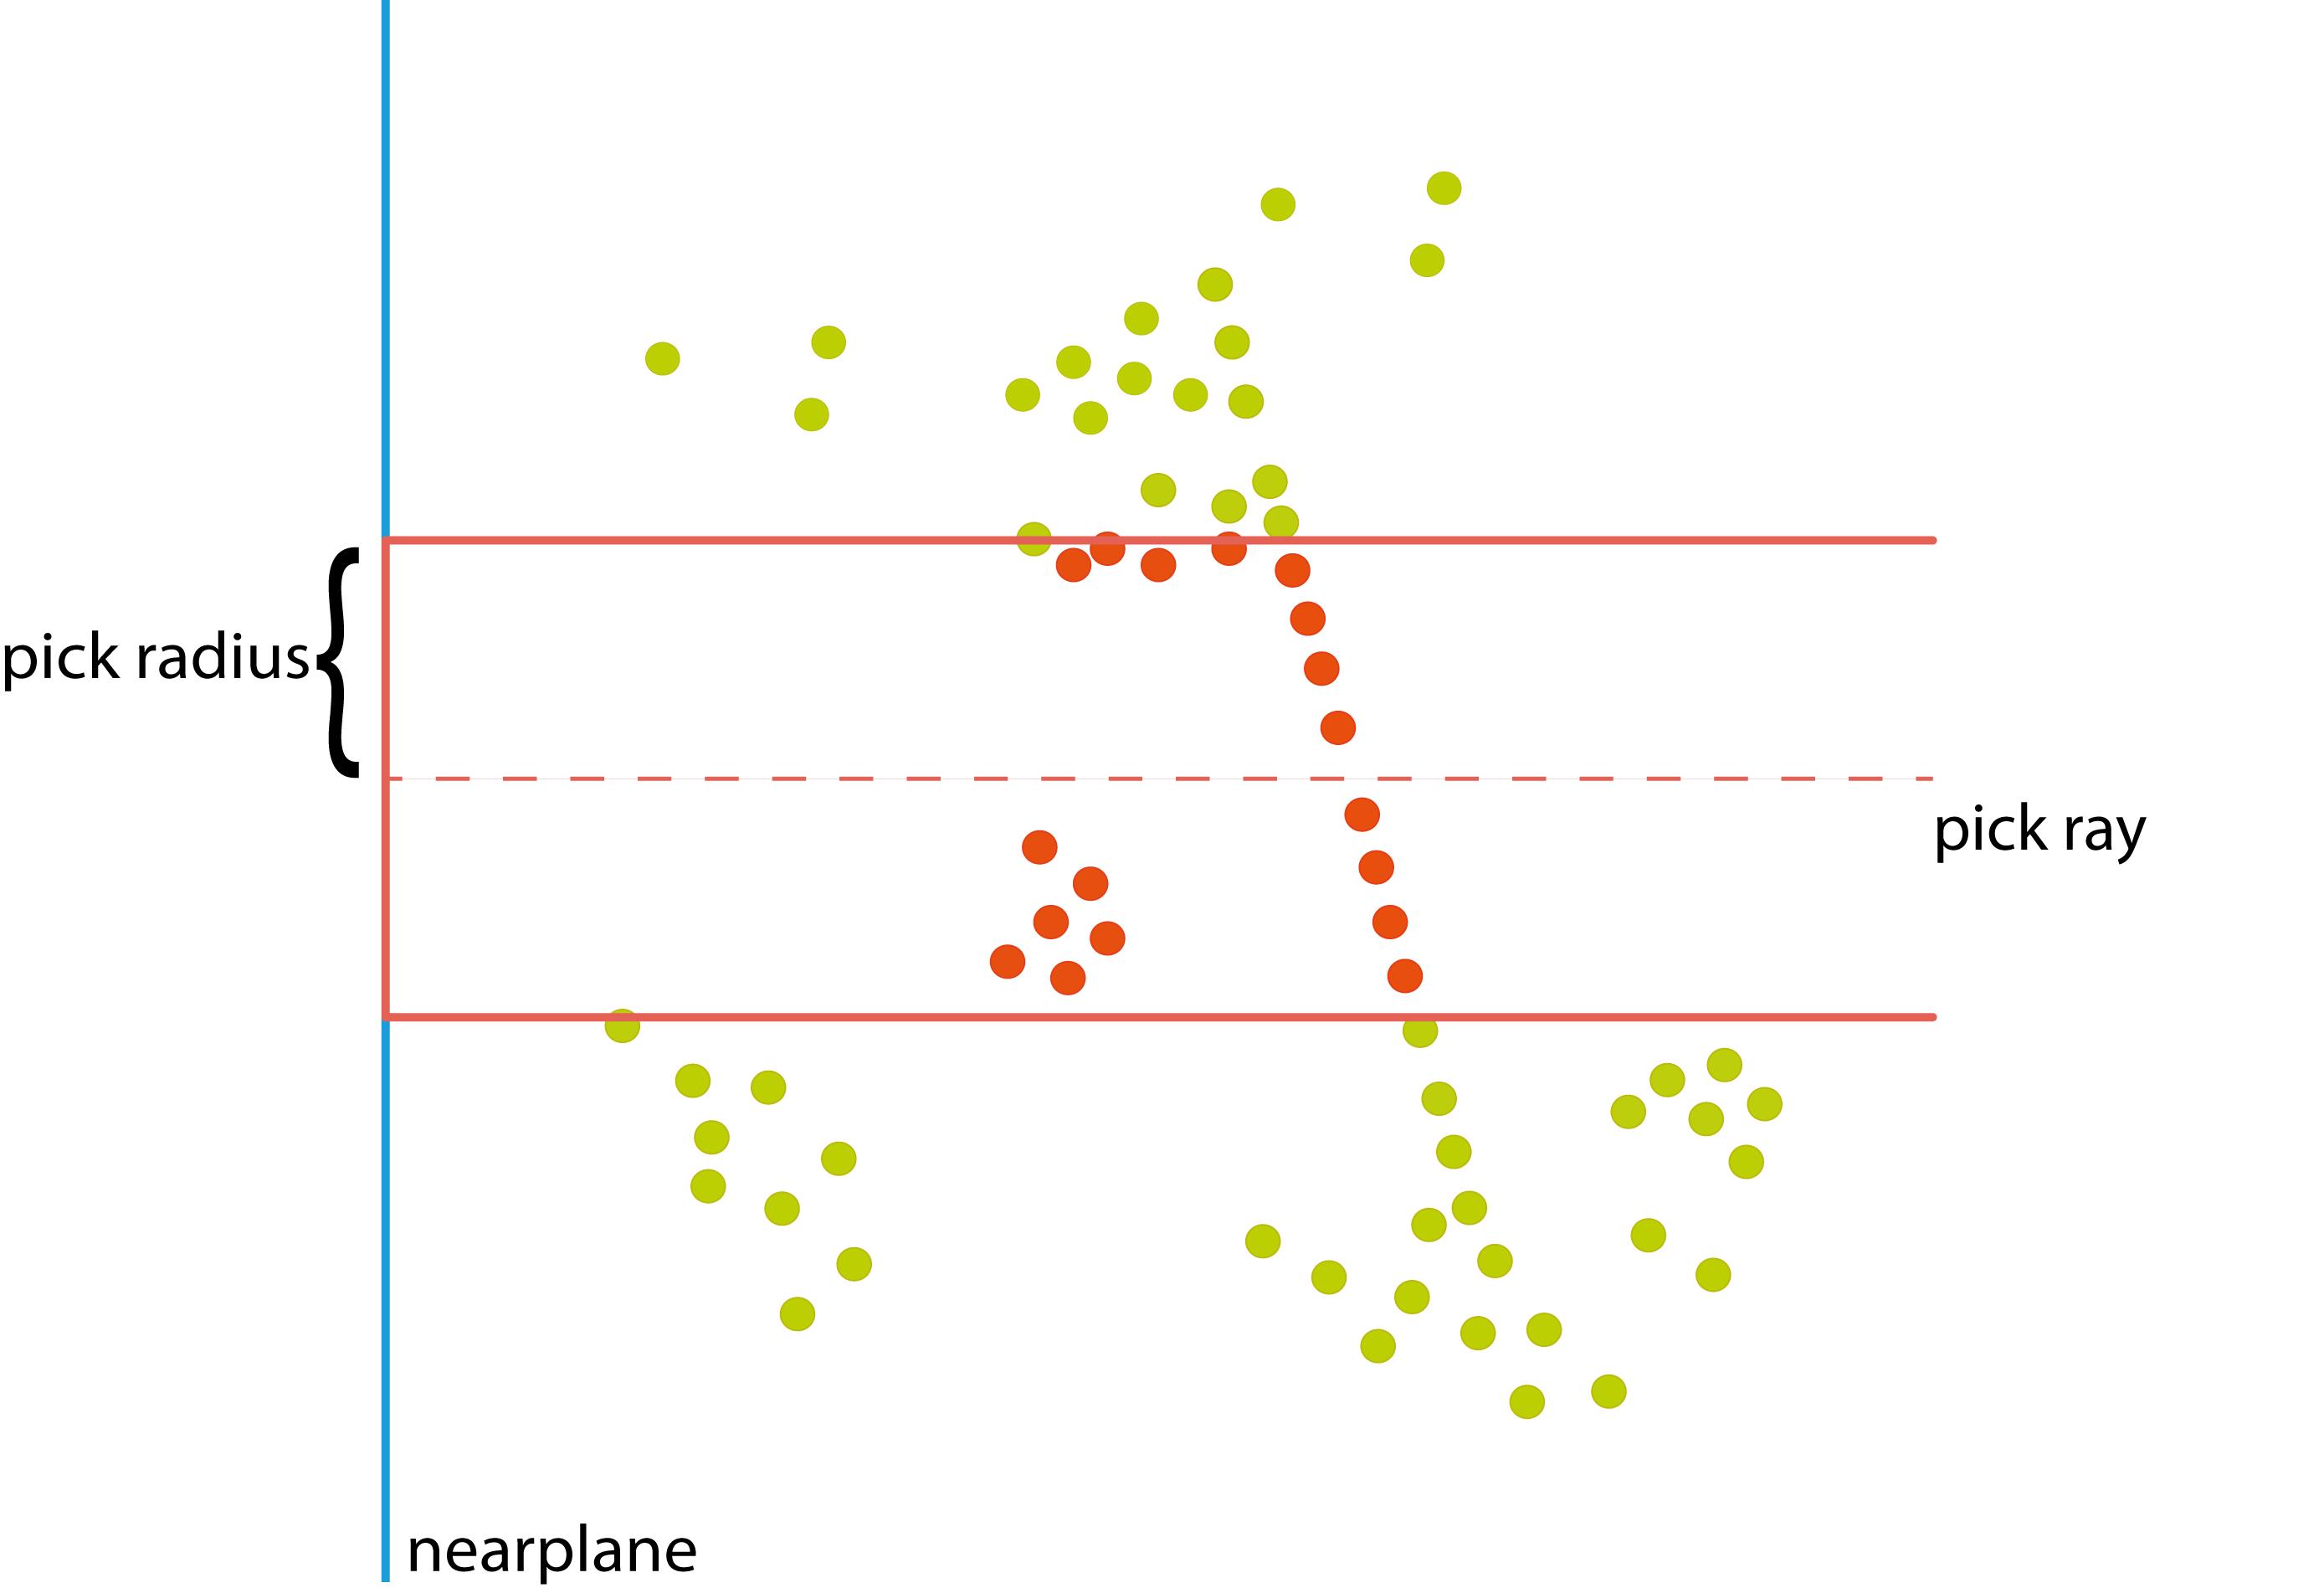
\includegraphics[width=0.6\textwidth]{System_Design/picking_raycast.png}%7
  }\par\medskip
\subcaptionbox{ \label{fig:picking_conecast}}{%
  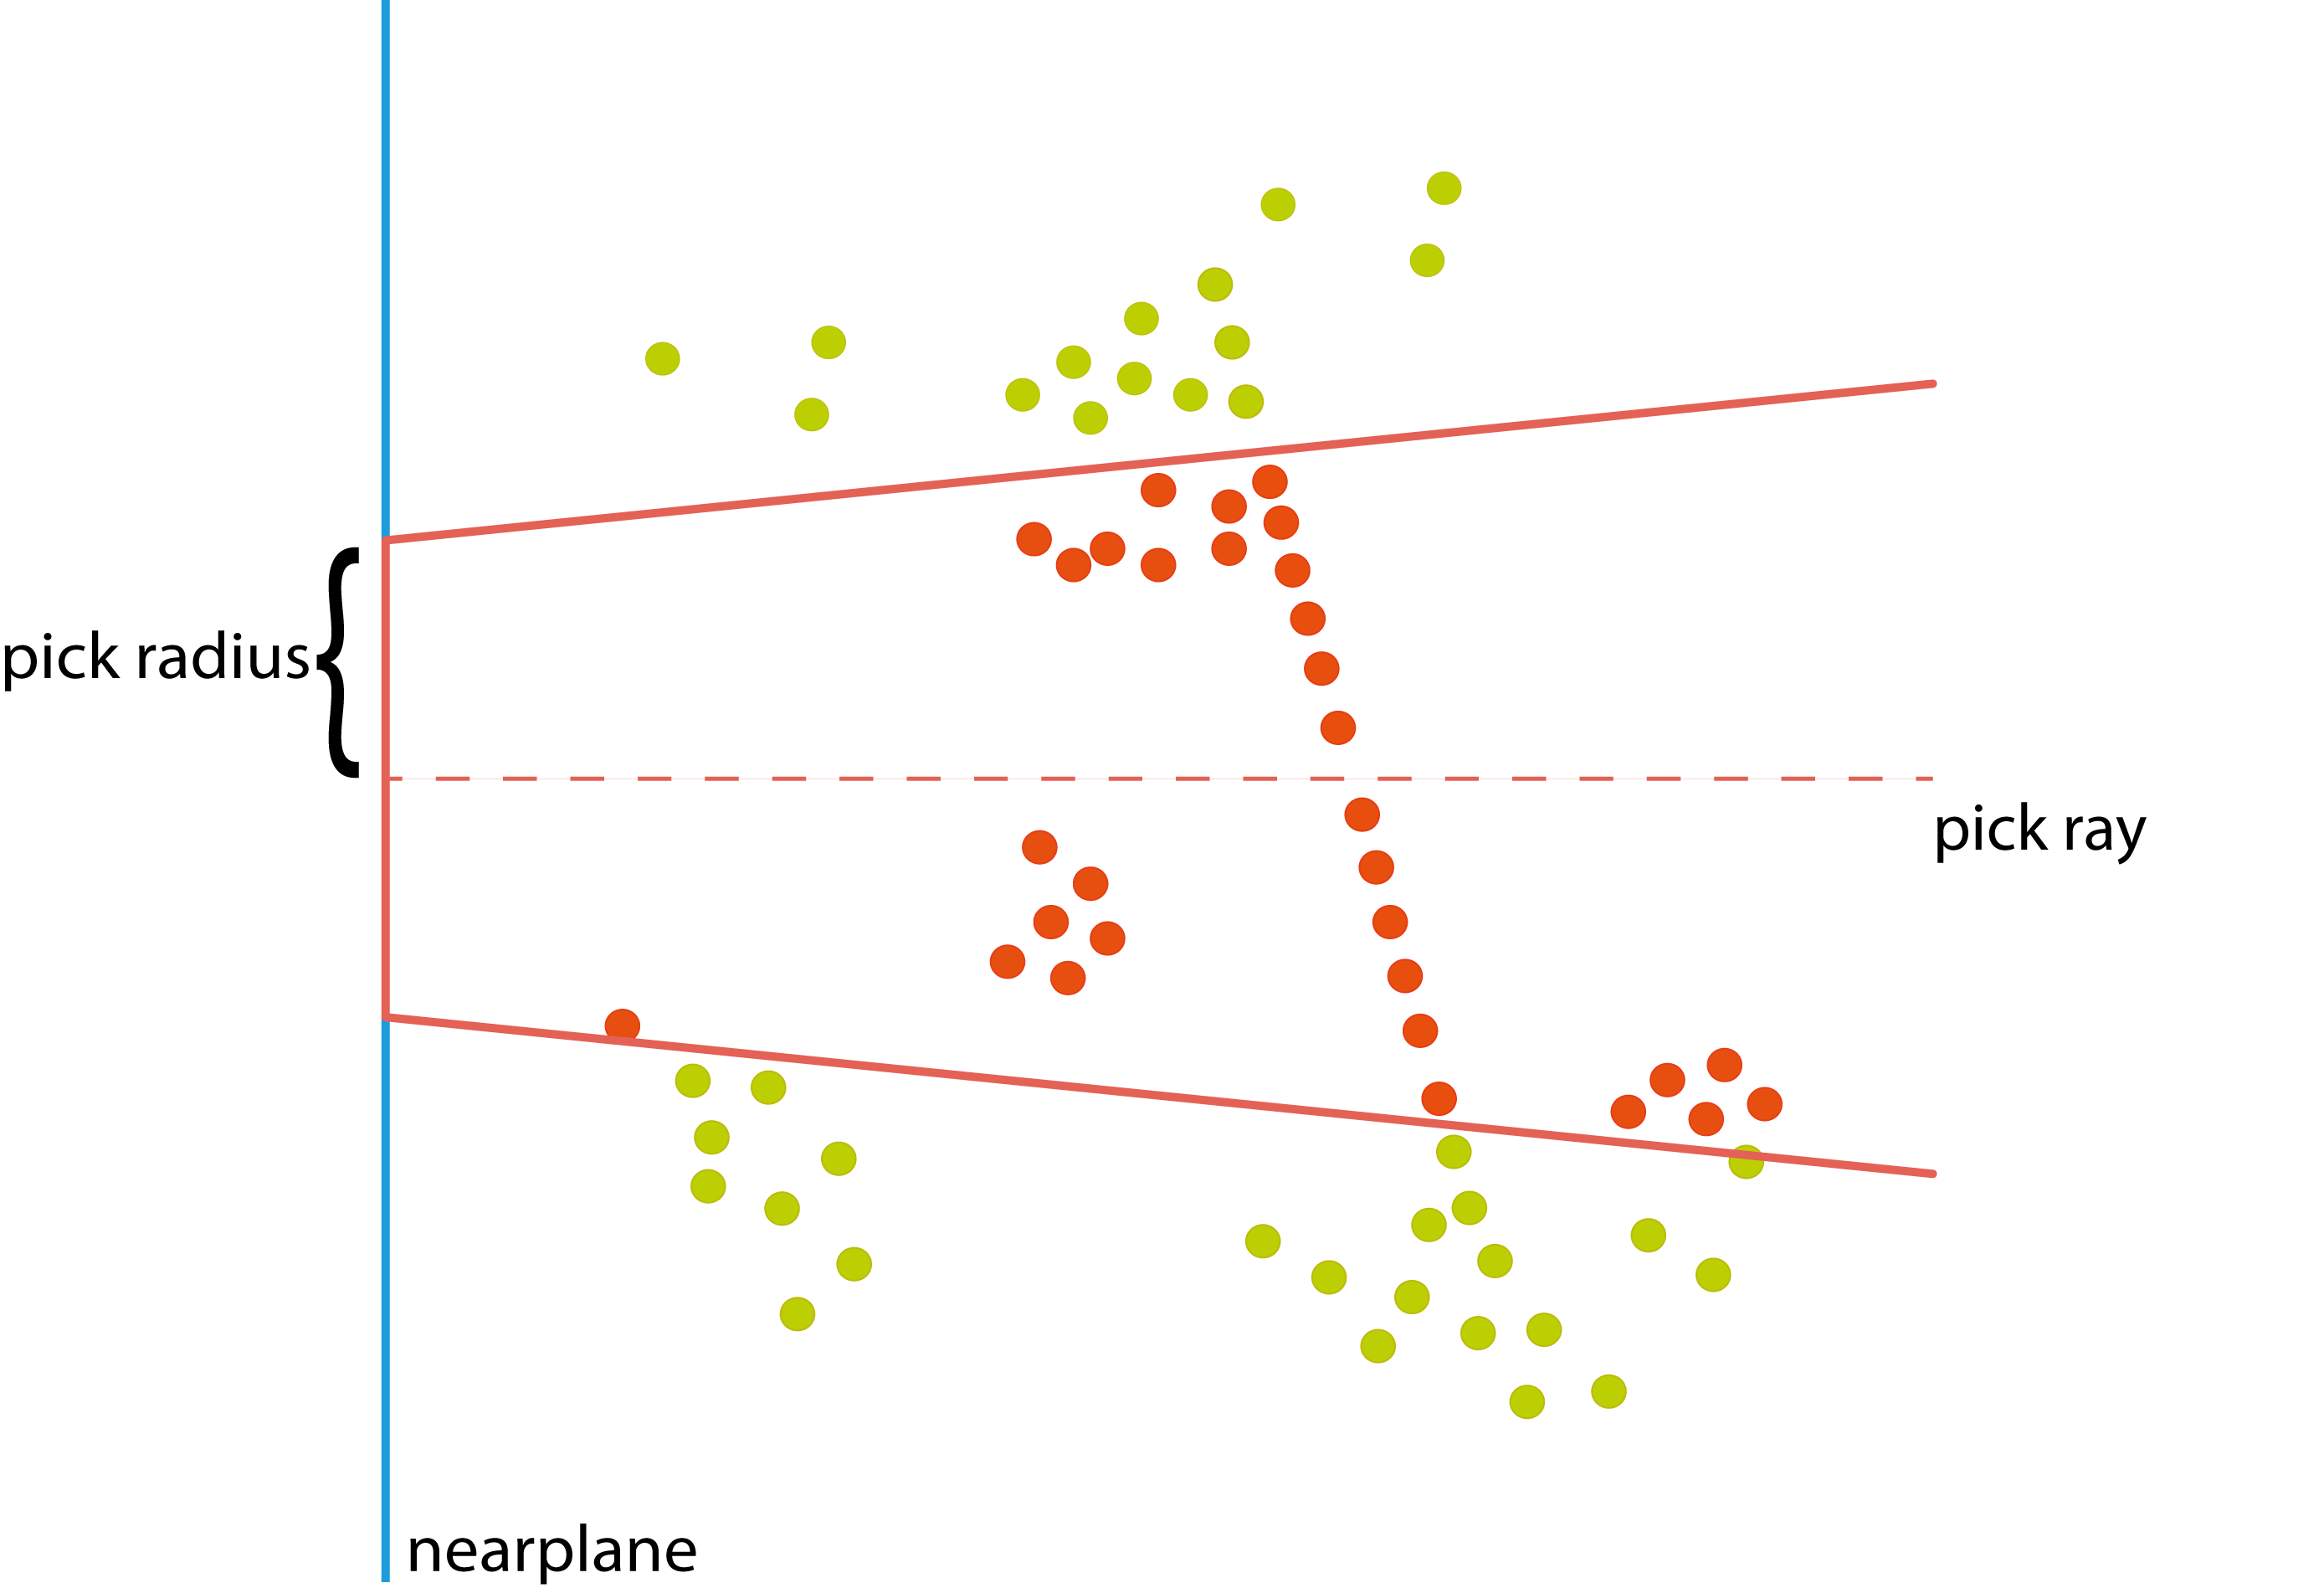
\includegraphics[width=0.6\textwidth]{System_Design/picking_conecast.png}%
  }\par\medskip        
\subcaptionbox{ \label{fig:picking_assisted}}{%
  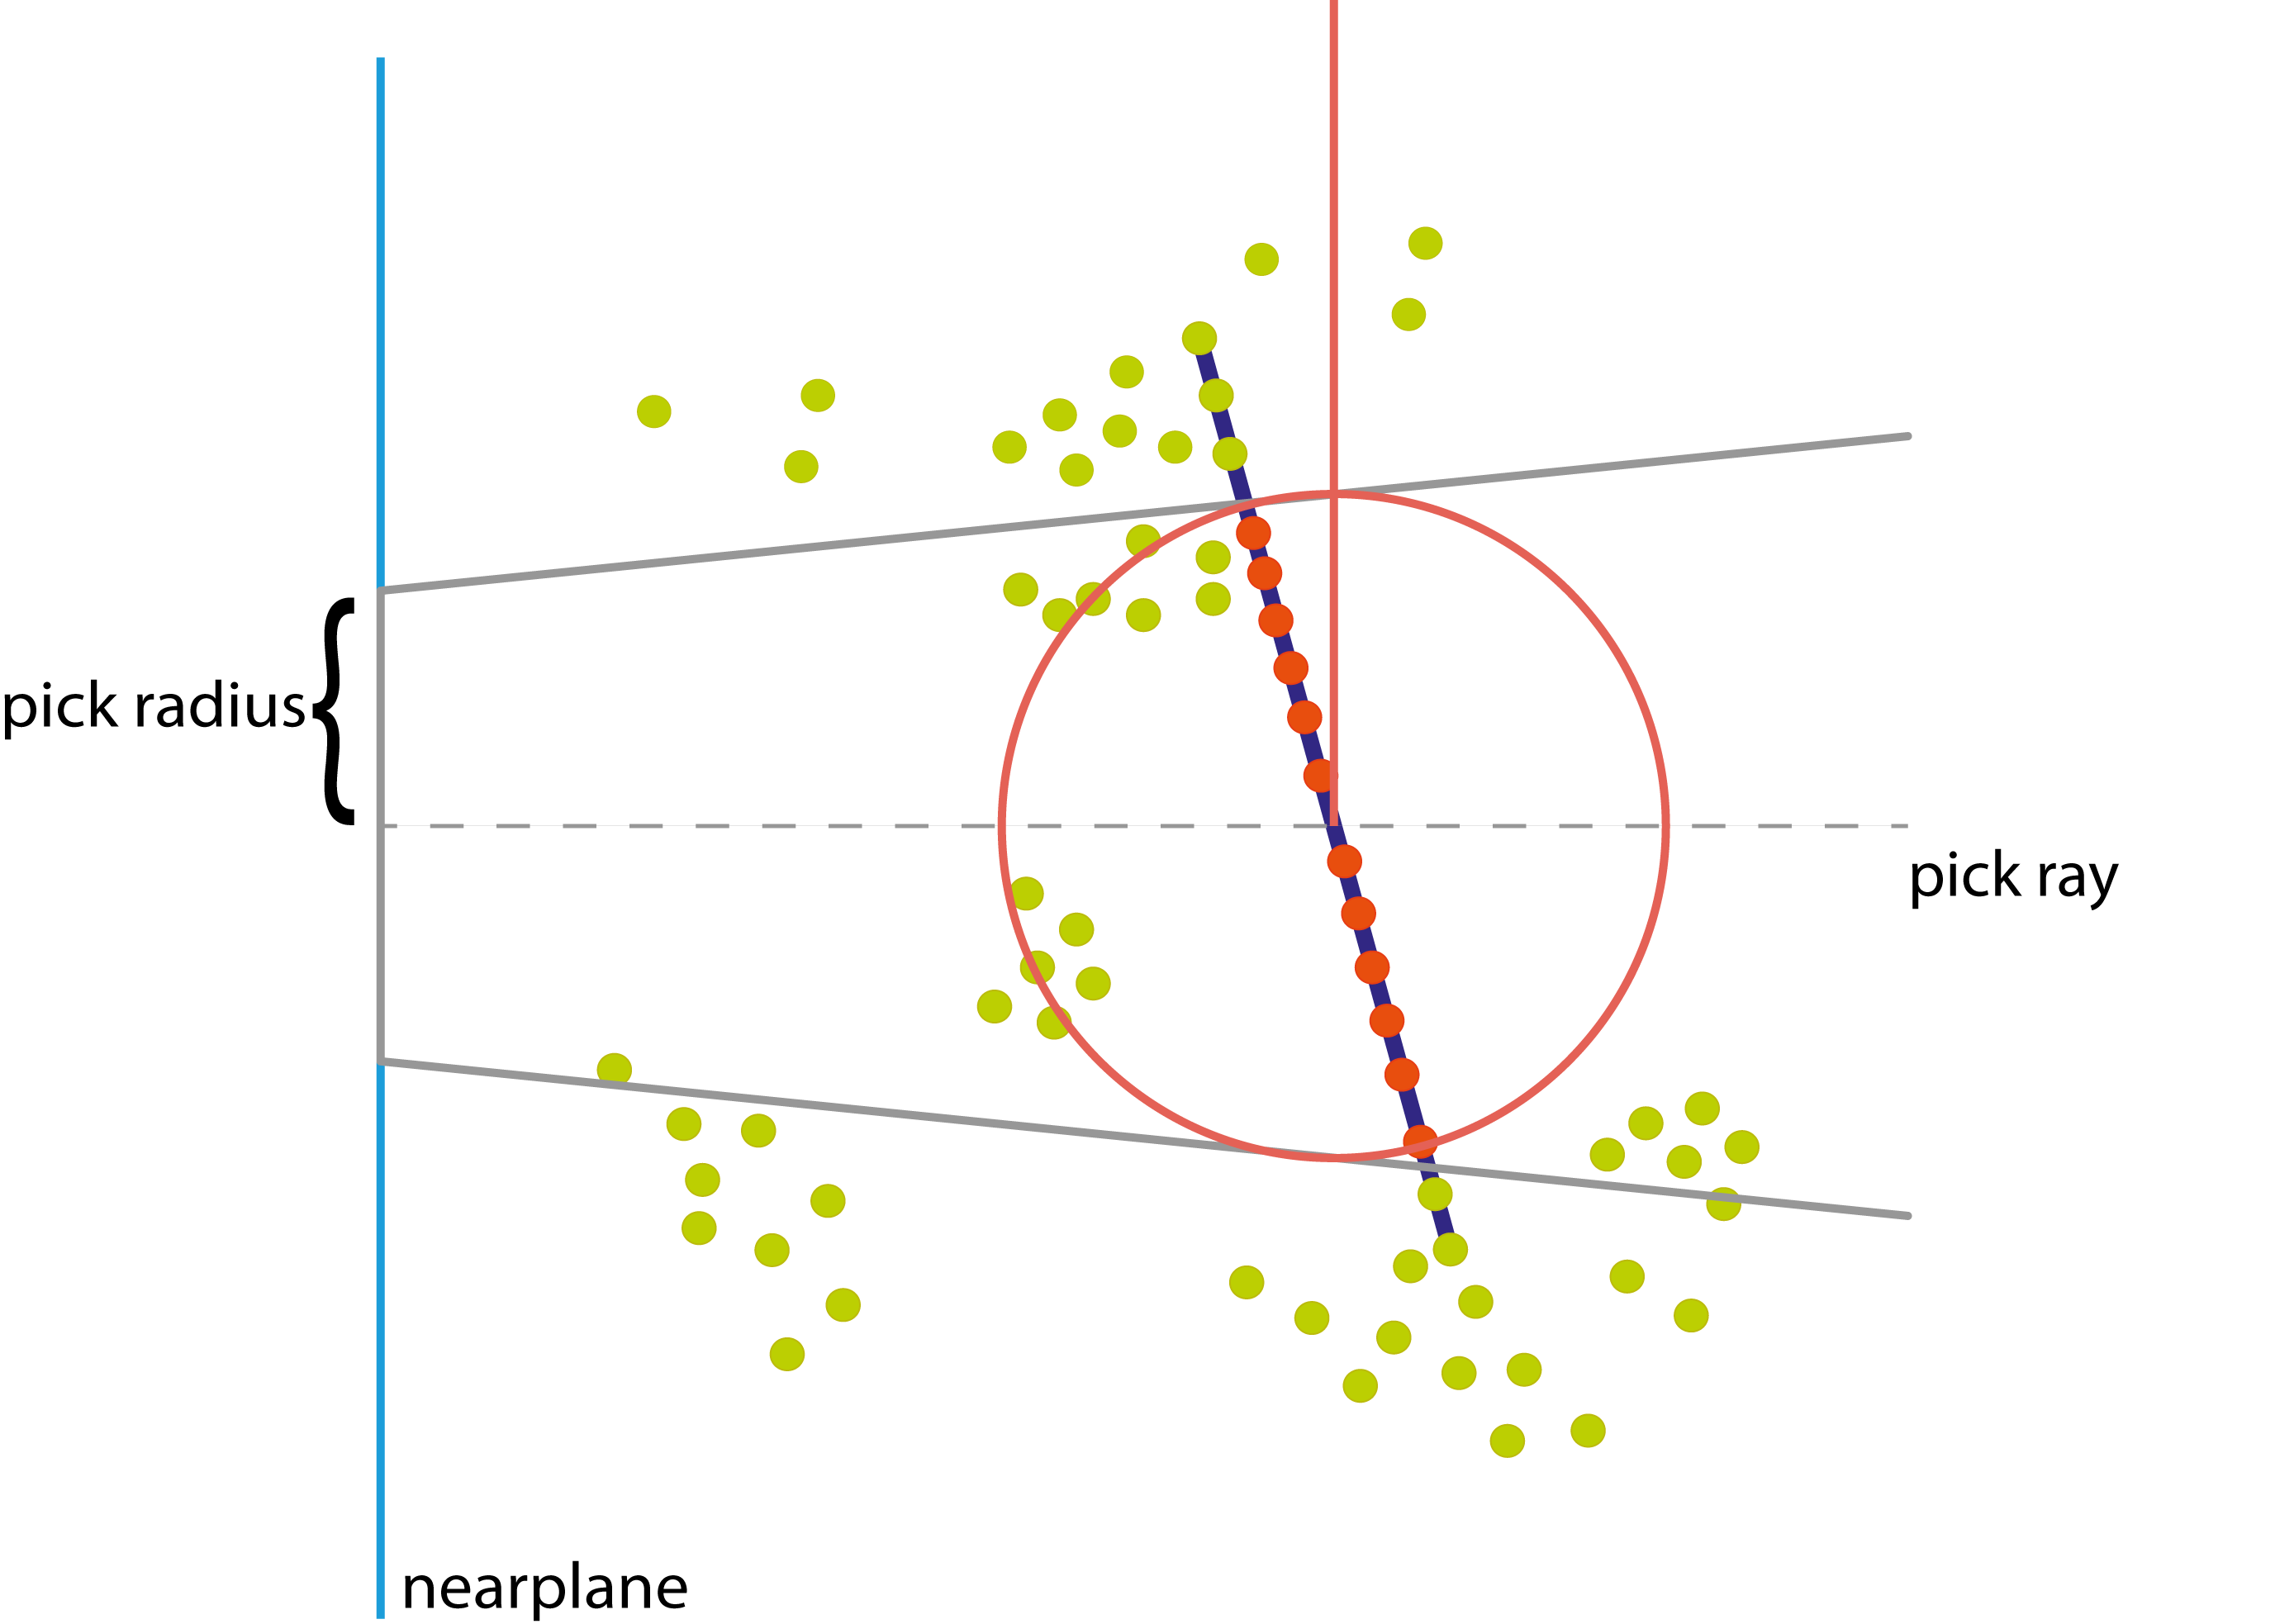
\includegraphics[width=0.6\textwidth]{System_Design/picking_assisted.png}%
  }
\caption{Two-dimensional illustration of various picking methods. Candidate points are colored in green; other points are colored in red. The areas in red describe the different volumes in which candidate points are located. (a) showcases a picking process using a simple raycast. The ray combined with a radius constructs a cylinder in world space which contains all candidate points, (b) uses a cone instead. (c) utilizes a selected shape (dark blue) to filter candidate points that follow the curvature of the shape. A spherecast is then performed on the filtered points using the unprojected pick radius to obtain the final set of candidate points. }
\label{fig:picking_overview}
\end{figure}


Figure \ref{fig:picking_overview} shows the different picking methods, described in Section \ref{sec:pointPicking}. Figure \ref{fig:picking_raycast} showcases a simple raycast with a radius. The combination of a ray and a radius yields a cylinder, which contains all candidate points on world space. The pick distance is consistent in world space. Figure \ref{fig:picking_conecast} uses a conecast instead. The opening angle is defined by the pick radius in screen space. The pick distance in world space increases the higher the depth value. All points inside the volume are treated equally, introducing consistency in screen space. Figure \ref{fig:picking_assisted} showcases the use of a support shape to filter candidate points. All points that belong to the support shape are filtered prior to being used as input for a spherecast. 


\begin{figure}
    \centering
    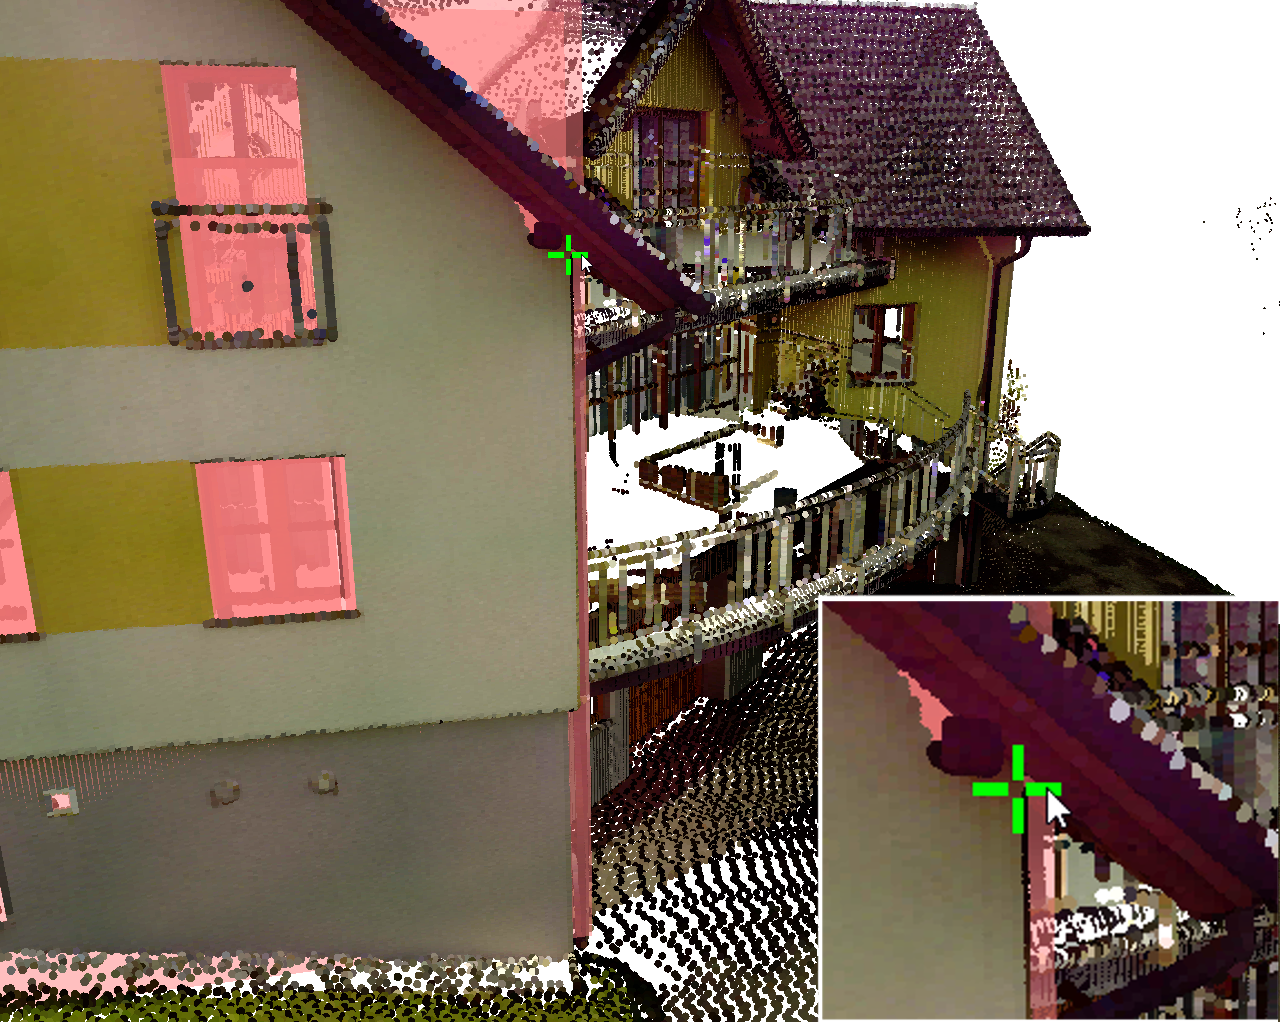
\includegraphics[width=0.8\textwidth]{System_Design/picking_assisted_screenshot.png}%7
    \caption{\textit{Shape-assisted Point Picking} is performed on a shape cluster that represents the wall in the foreground. The cross hair indicates the picked point. Note that the cross hair does not jump to a point in the background even though they would be closer to the cursor in screen space. }
    \label{fig:picking_assisted_screenshot}
\end{figure}

The result of \textit{Shape-assisted Point Picking} can be seen in Figure \ref{fig:picking_assisted_screenshot}. The crosshair, even though other points' projections are closer to the cursor, sticks to the structure. Picking points on edges is improved in particular since the picking result follows the edge rather than jumping to a point in the background. 


\subsection{Region Selection}
\label{sec:regionSelection}

Region Selection aims to select a set of points, that share certain criteria, rather than picking a single point. 
The design for the \textit{Shape-Assisted Region Selection} is guided by one seemingly simple example task: \textit{Select points that belong to this wall only}. A wall can intersect with other building elements such as roof, balconies or the ground. In regions close to intersections, it is tedious and cumbersome to only select points on the desired structure. Using two-dimensional interaction metaphors, selecting multiple spatially neighboring points along the same curvature is particularly challenging due to the system not knowing the desired depth boundaries for the selection region. In this section, the benefits of using support shapes for two- and three-dimensional interaction metaphors to select regions of points,  are discussed. 


\subsubsection{Lasso Selection}

The \textit{Lasso Selection} is a common two-dimensional interaction metaphor used for multiple geometry-based applications. While it is a useful technique to selected regions in 2D, drawbacks appear when porting the interaction to 3D. The user draws a polygon onto the screen. All points, whose projection lie inside this polygon, are selected. Much like \textit{Point Picking}, points are projected onto the nearplane, the intersection between the point and the lasso polygon in screen space determines whether a point is selected. The lasso polygon in combination with the camera view creates a three-dimensional volume, whose area contains all points whose projection lie inside the lasso polygon. Figure \ref{fig:lasso_sketch} showcases the volume created by a lasso polygon drawn onto the screen.

Note that this interaction is computed asynchronously and the selection is performed on the complete octree. Therefore, it is essential that octree nodes, whose \textit{level-of-detail} are too high and therefore are not rendered, are still included in this interaction as well. 


\begin{figure}
    \centering
    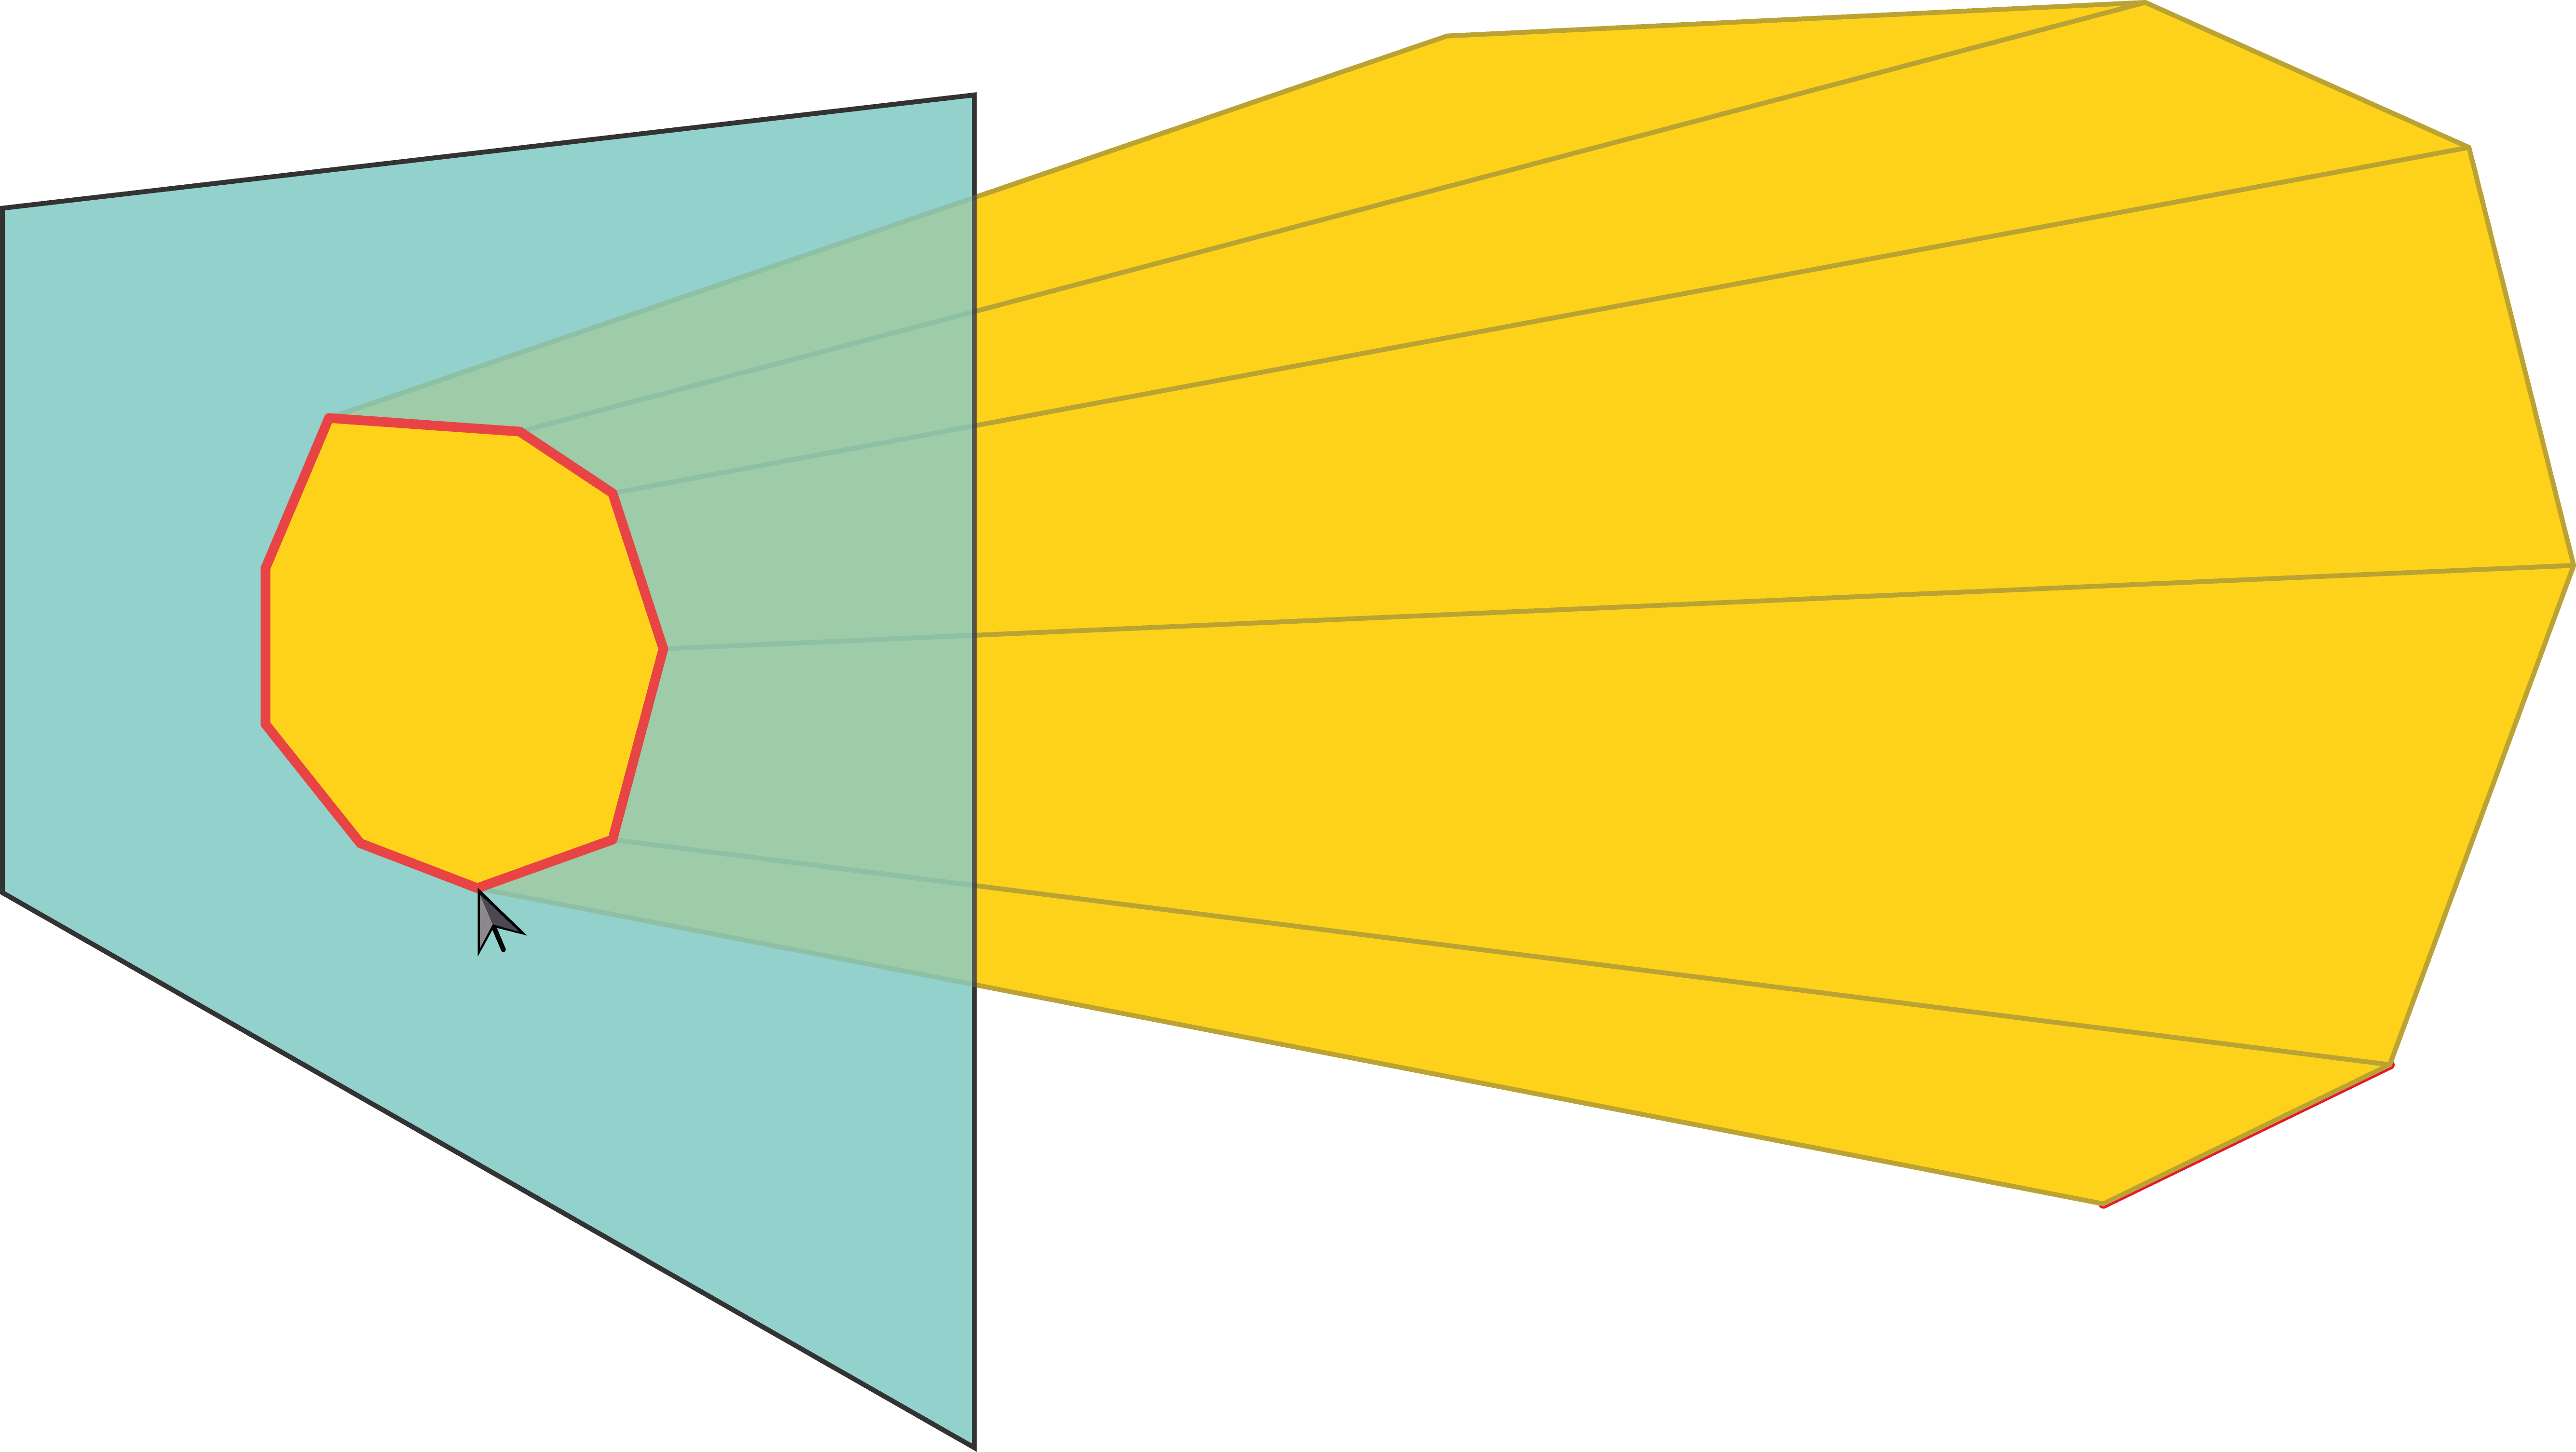
\includegraphics[width=0.8\textwidth]{System_Design/lasso_sketch.png}%7
    \caption{The user draws a polygon(red) on the screen(light blue). The constructed three-dimensional area(yellow) contains all points, whose projection lie inside the lasso polygon. }
    \label{fig:lasso_sketch}
\end{figure}


\begin{figure}
\centering
\subcaptionbox{ \label{fig:lasso1}}{%
  \includegraphics[width=0.5\textwidth]{System_Design/lasso1.png}%7
  }\par\medskip
\subcaptionbox{ \label{fig:lasso2}}{%
  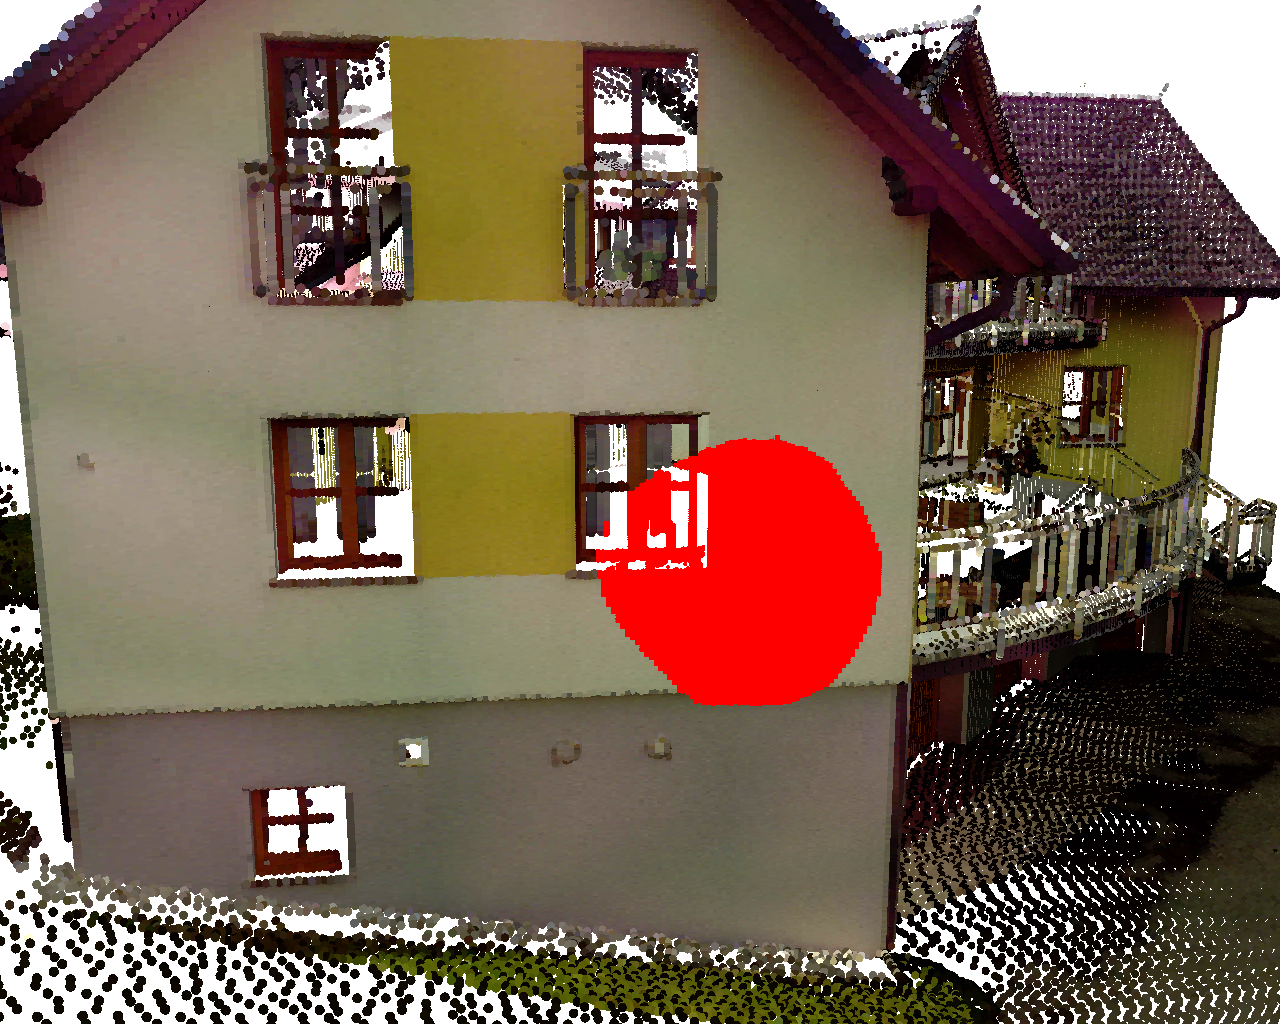
\includegraphics[width=0.5\textwidth]{System_Design/lasso2.png}%
  }\par\medskip        
\subcaptionbox{ \label{fig:lasso3}}{%
  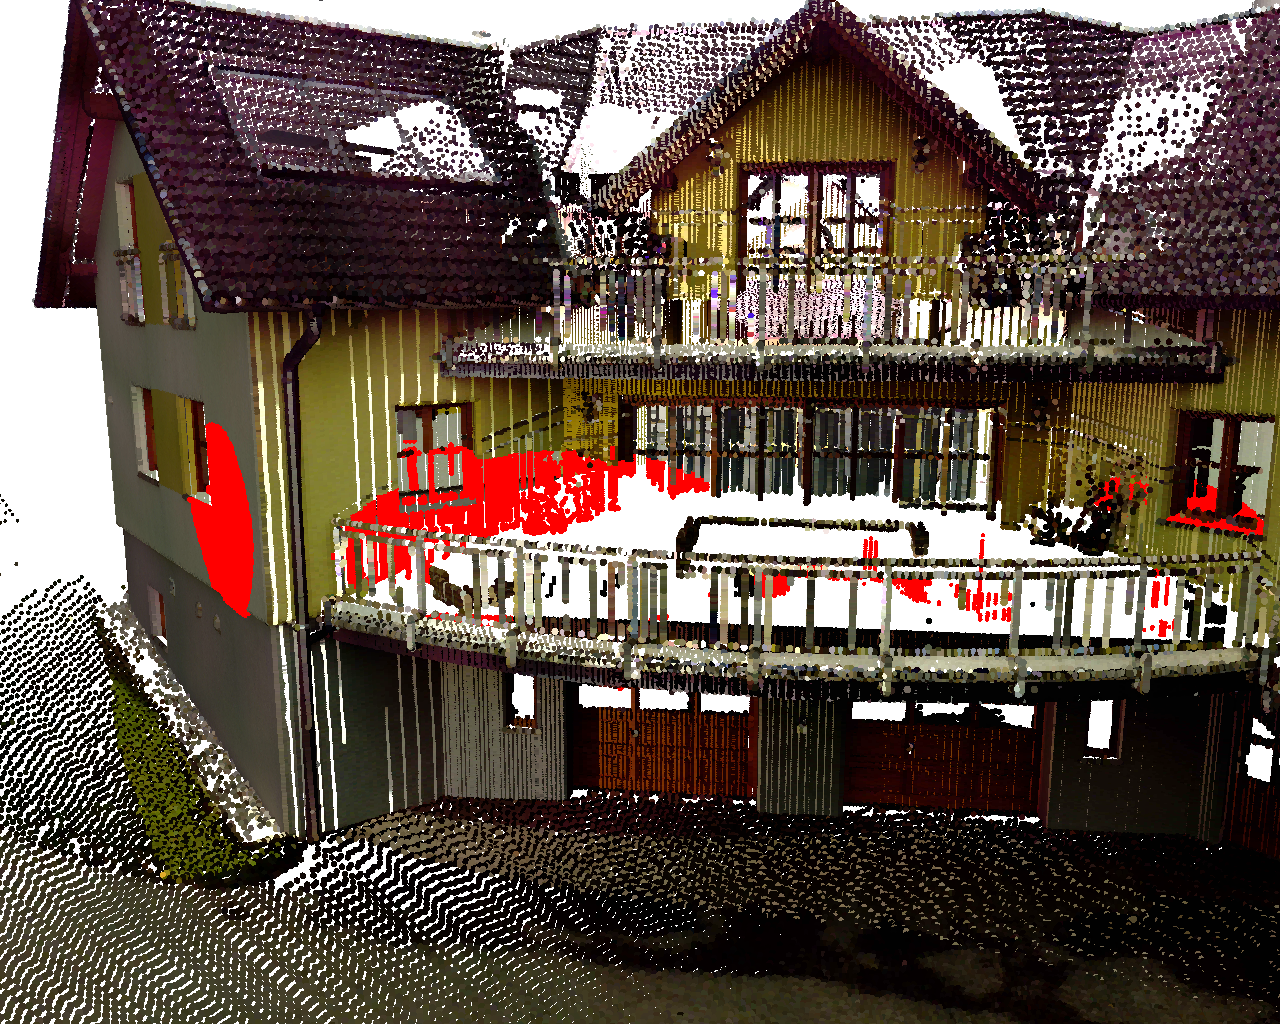
\includegraphics[width=0.5\textwidth]{System_Design/lasso3.png}%
  }
\caption{(a) - (c) show a lasso selection performed on a point cloud. In (a) the user draws a polygon onto the screen. In (b) the selected points are visualized in red. Figure (c) showcases the selection from a different angle. All points that are projected to the area of the polygon are selected.The unintentional selection of points that are obscured by objects in the foreground is a byproduct of the \textit{Lasso Selection}. }
\label{fig:lasso}
\end{figure}


Figure \ref{fig:lasso} shows a lasso selection performed on a point cloud. The user draws a polygon onto the screen. The selected points are highlighted in red. When changing the view, selected points that were occluded while drawing the lasso, appear. The user must control the selection distance by hand to minimize this effect. However, to solve the task of only selecting points on the wall, further lasso selections must be applied to remove points from the selection that were selected unintentionally. 


\subsubsection{Shape-Assisted Lasso Selection}

The aim of this interaction is to provide a smaller set of points on which a \textit{Lasso Selection} is performed.  The octree nodes are again filtered using the technique described in Section \ref{sec:pointFiltering} to reduce the number of candidate nodes and points. On this reduced set, a \textit{Lasso Selection} is performed. The result of this interaction is a selection that mimics a \textit{Lasso Selection}, with the benefit of not selecting 'through' the point cloud. The depth ambiguities of the \textit{Lasso Selection} are circumvented by introducing continuous depth boundaries defined by the local curvature of the shape cluster. 

Figure \ref{fig:lasso_assisted} shows the workflow for selecting points on a shape. The shape is selected beforehand by the user. A lasso is drawn on the screen which selects all points that lie within the lasso and belong to the selected support shape. In Figure \ref{fig:lasso_assisted3}, it can be seen that contrary to Figure\ref{fig:lasso3}, no points are selected that do not belong to the support shape.

\begin{figure}
\centering
\subcaptionbox{ \label{fig:lasso_assisted1}}{%
  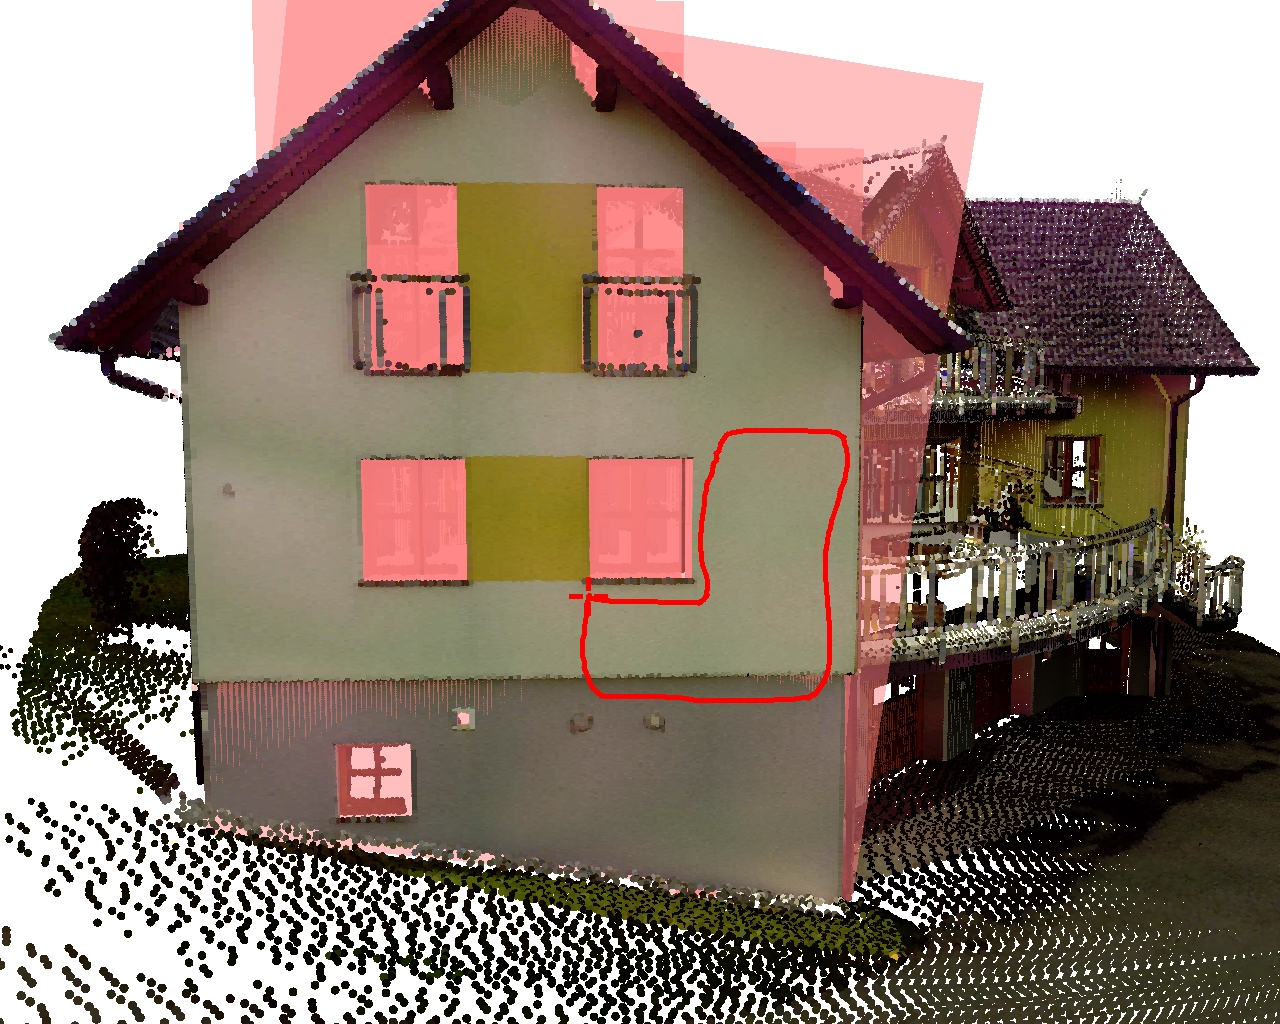
\includegraphics[width=0.5\textwidth]{System_Design/lasso_assisted1.png}%7
  }\par\medskip
\subcaptionbox{ \label{fig:lasso_assisted2}}{%
  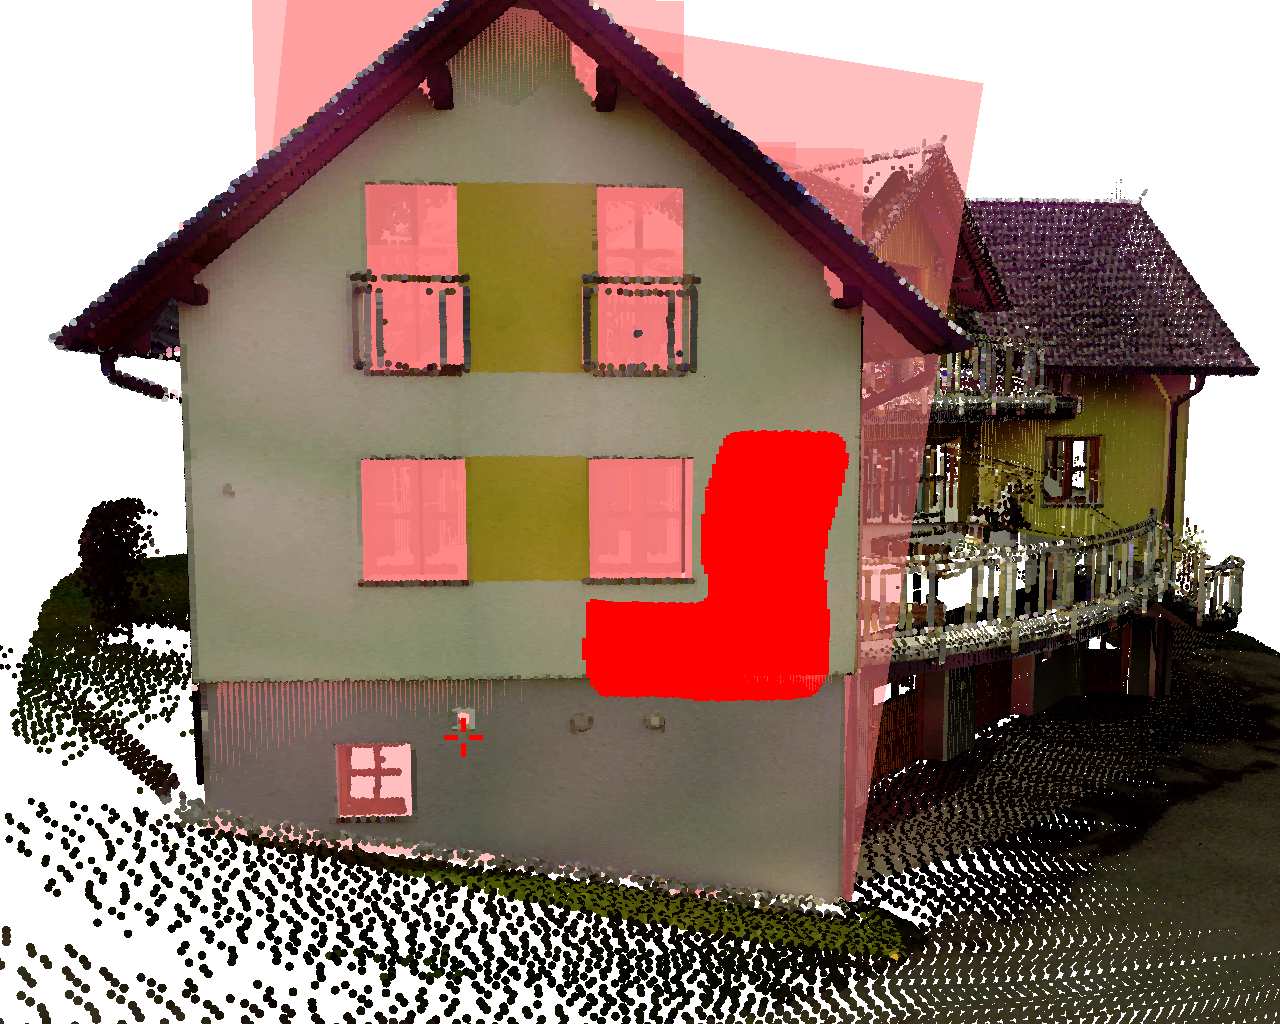
\includegraphics[width=0.5\textwidth]{System_Design/lasso_assisted2.png}%
  }\par\medskip        
\subcaptionbox{ \label{fig:lasso_assisted3}}{%
  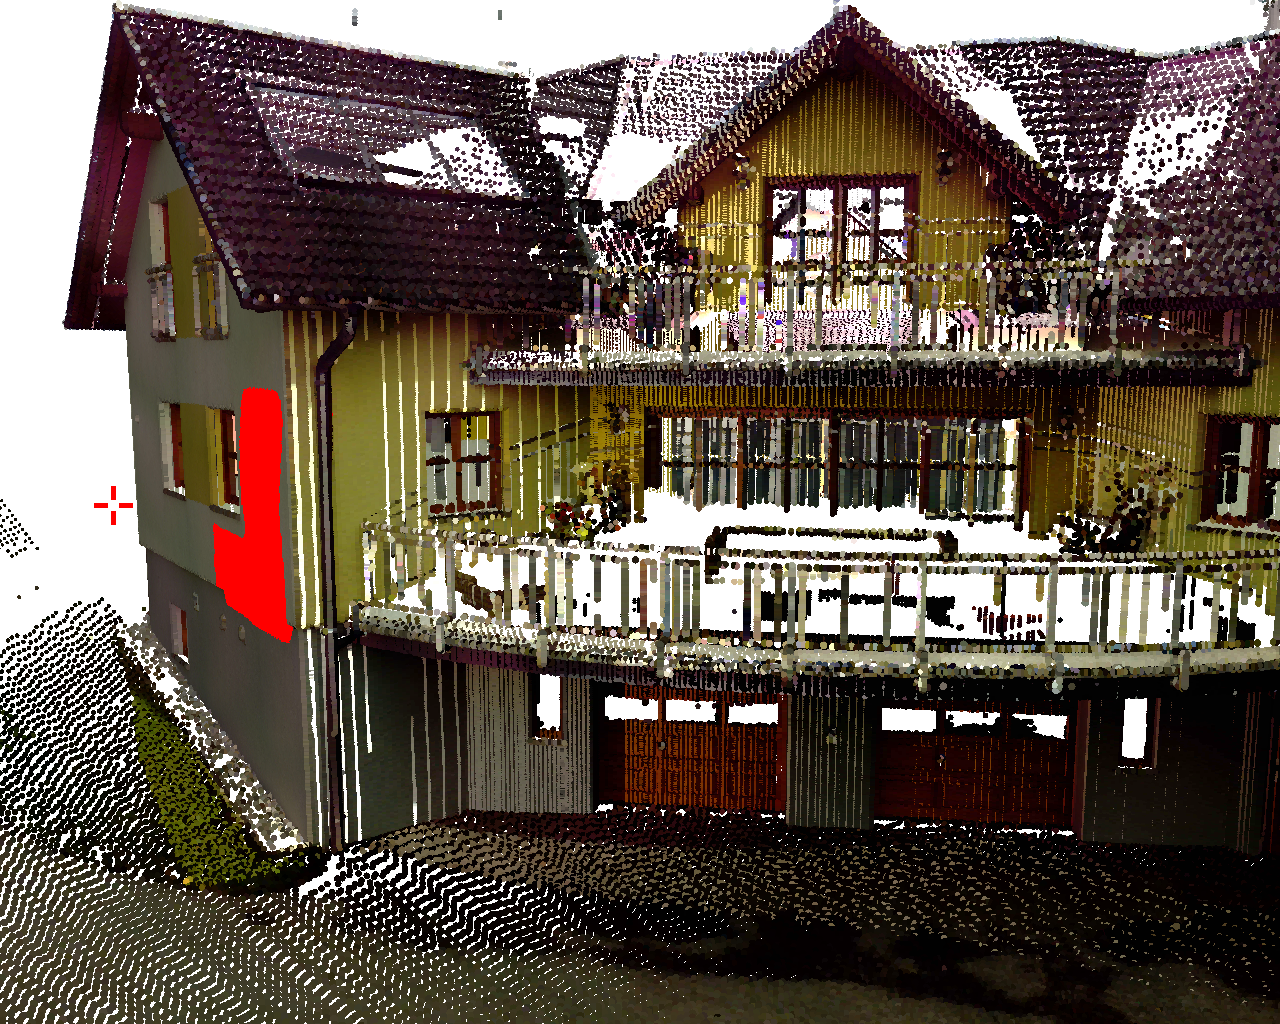
\includegraphics[width=0.5\textwidth]{System_Design/lasso_assisted3.png}%
}
\caption{(a) - (c) show a \textit{Shape-Assisted Lasso Selection} performed on a point cloud. The front facing wall is selected as support shape by the user. The shape cluster is visualized in light red. In (a) the user draws a polygon onto the screen after selecting a shape as support shape. (b) shows the selected points visualized in red from the same point of view. Upon view change, it can be seen that this interaction only selects points that belong the shape cluster. }
\label{fig:lasso_assisted}
\end{figure}


\subsubsection{Volumetric Brush}

The \textit{Volumetric Brush} by Weyrich et al. \cite{weyrich2004post} is designed in such a way that a volume is projected onto the foremost geometry. Points that intersect this volume are considered to be selected. To retrieve the projected position of the volume, usually a sphere, the depth buffer is consulted, and the depth value for the current mouse position is retrieved. The world position is the unprojection of the mouse position's $xy$-coordinates and the depth value. 
\\
Since this technique follows the foremost geometry only, sudden depth changes occur if different geometry occludes the area of interest. Thus, view changes are still required to achieve the example task. In regions close to intersections with other structures, such as below the roof, the user must control the size of the volume to not select points on neighboring structures. 


\subsubsection{Shape-Assisted Volumetric Brush}

The \textit{Volumetric Brush} can easily be adapted to be used in combination with support shapes. Instead of consulting the depth buffer to reconstruct the cursor’s world position, the pick ray is intersected with the selected support shape, thus resulting in a three-dimensional world position. The selection is then performed only on the filtered set of points as described in Section \ref{sec:pointFiltering}. 
Figure \ref{fig:brush} shows a \textit{Shape-Assisted Volumetric Brush} interaction performed on a wall. The wall creates as a cluster of planes. Only points are selected that belong to this cluster. 

\begin{figure}
\centering
\subcaptionbox{ \label{fig:brush_assisted1}}{%
  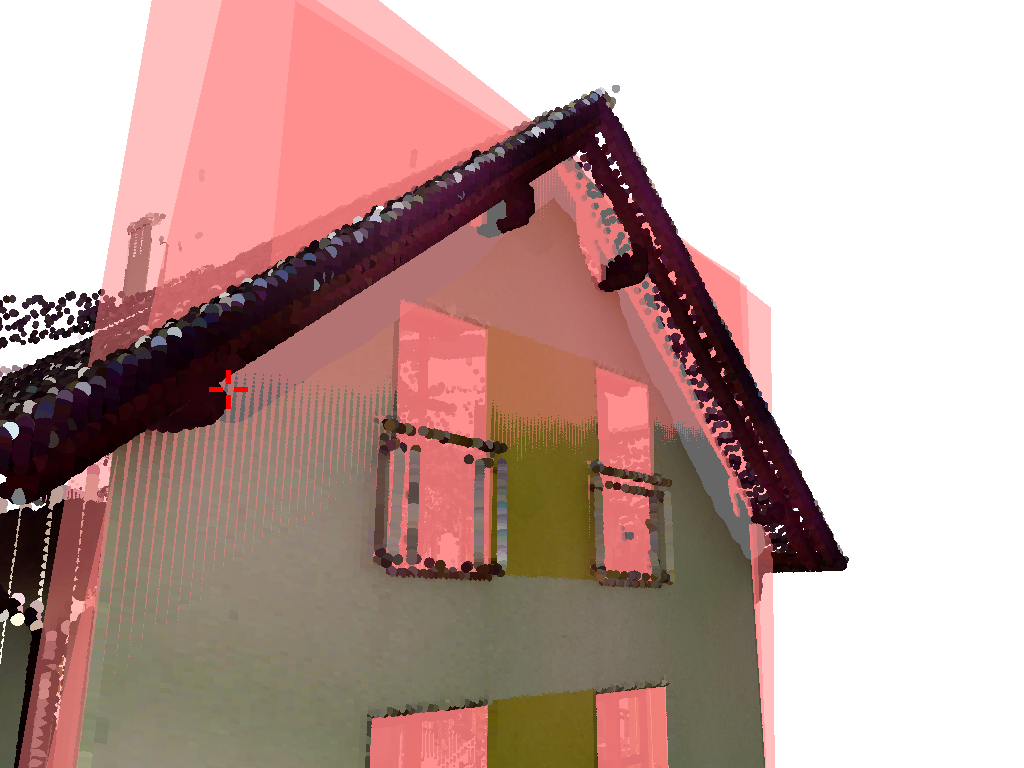
\includegraphics[width=0.8\textwidth]{System_Design/brush1.png}%7
  }\par\medskip
\subcaptionbox{ \label{fig:brush_assisted2}}{%
  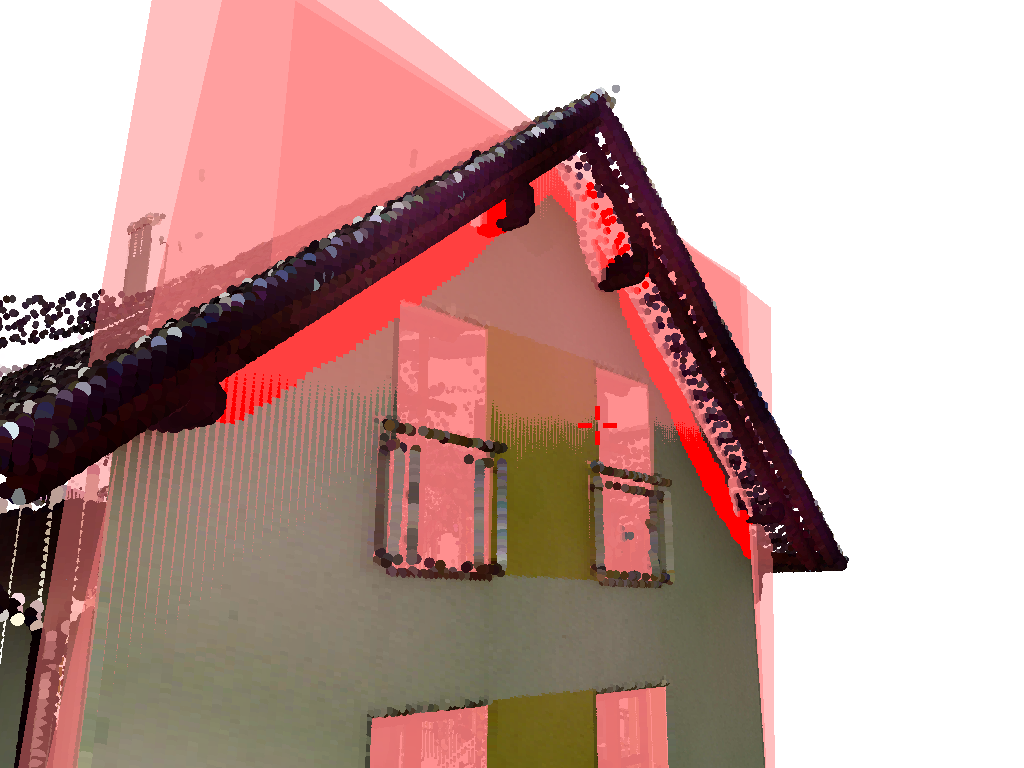
\includegraphics[width=0.8\textwidth]{System_Design/brush2.png}%
  }
\caption{This figure shows a \textit{Shape-Assisted Volumetric Brush} selection performed shape cluster (transparent red) detected in a point cloud. In (a) the trajectory of the brush is shown as subsequently rendered spheres(grey). (b) shows the selected points for this brush interaction. Even tough some points of the roof structure are intersecting the brush, they are not selected. }
\label{fig:brush}
\end{figure}


\subsection{Shape-Assisted Local Level-of-Detail Increment}
\label{sec:lod_increment}

To further investigate the local structures of a point cloud, the currently rendered maximum level-of-detail might not suffice. The highest \textit{level-of-detail} is chosen such, that the GPU is not overloaded and the balance between detail and performance is retained. However, temporarily adding a handful of additional nodes is sufficient enough to provide more detailed information, that can be presented without an enormous impact on performance.
\\

Section \ref{sec:renderHorizon} describes the set of nodes that are still rendered, but where some of the children are not rendered anymore, as \textit{render horizon}. 
Increasing the \textit{level-of-detail} is only useful for nodes that lie on the \textit{render horizon}. Beyond these nodes, more detailed information exists that is currently not rendered. A raycast is performed on the render horizon. All nodes that intersect the ray are considered to be candidate nodes. The successor nodes of the candidate nodes hold more detailed information on the region of interest. Depending on a \textit{level-of-increment} parameter, controlled by the user, the successors of those nodes are added to the scene and rendered. A \textit{level-of-increment} value of $1$ results in adding all children for each node on the render horizon, a parameter of $2$ results in adding all children's children to the scene. 
By adding smaller nodes of higher level-of-detail, the overall detail in the scene is amplified. However, by plainly adding additional nodes, noise and unwanted structures are amplified as well. 
\\

\textit{Shape-Assisted Local Level-of-Detail Increment} utilizes a selected shape cluster to amplify detail only on structures of interest. The user selects a primitive shape as support shape. Instead of performing a raycast, the nodes on the render horizon that intersect the support shape, are collected. From these nodes, only those points that belong to the support shape, are added to the scene. The membership of a point to the shale cluster is determined by the score function described in Section \ref{sec:scorefun}. 

\begin{figure}
\centering
\subcaptionbox{ \label{fig:lod_increment1}}{%
  \includegraphics[width=0.8\textwidth]{System_Design/lod_Increase.png}%7
  }\par\medskip
\subcaptionbox{ \label{fig:lod_increment2}}{%
  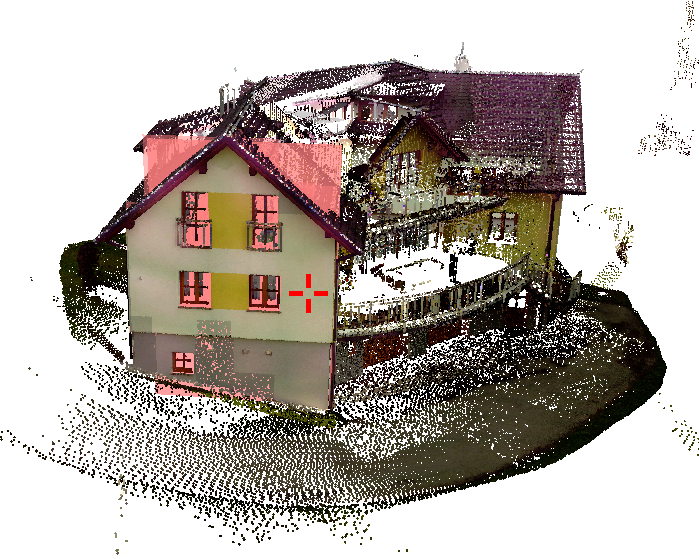
\includegraphics[width=0.8\textwidth]{System_Design/lod_Increase2.png}%
  }
\caption{This figure shows the benefits of \textit{Shape-Assisted Level-of-Detail Increment} for a point cloud. (a) shows the currently rendered structure, as well as as shape cluster that is currently selected (red). (b) shows the scene with amplified details along the structure. The additional points are rendered without lighting to appear brighter.}
\label{fig:lod_increment}
\end{figure}

Figure \ref{fig:lod_increment} showcases the difference in a scene with- and without amplified details along a wall. The selected support shape is rendered in transparent red, while the additional points are rendered without lighting to appear brighter. In the intersecting octree nodes, only those points are rendered that fulfill the shape's score function. 


